\chapter{Results}\label{chap:results}

\section{Total energy as a function of time for different time steps}
    \graphicspath{ {./figures/milestone04/} }
    \begin{figure}[!htb]
    % \captionsetup{justification=centering,margin=2cm}
    \centering
        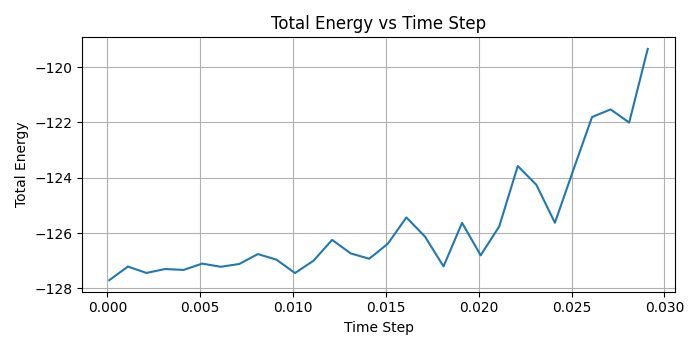
\includegraphics[scale=0.9]{total_energy_vs_time_step.png}
        \caption[Total energy vs Time steps using parameters]{\textbf{Total energy vs Time steps using parameters: start\_time\_step=1e-4, end\_time\_step=30e-3,step=1e-3, sigma=1, mass=1, epsilon=1, total\_time=5000}}
    \label{fig:total_energy_vs_time_step}
    \end{figure}


\section{Snapshots sequence of LJ simulation}
    \graphicspath{ {./figures/milestone04/} }
    \begin{figure}[h]

    \centering
        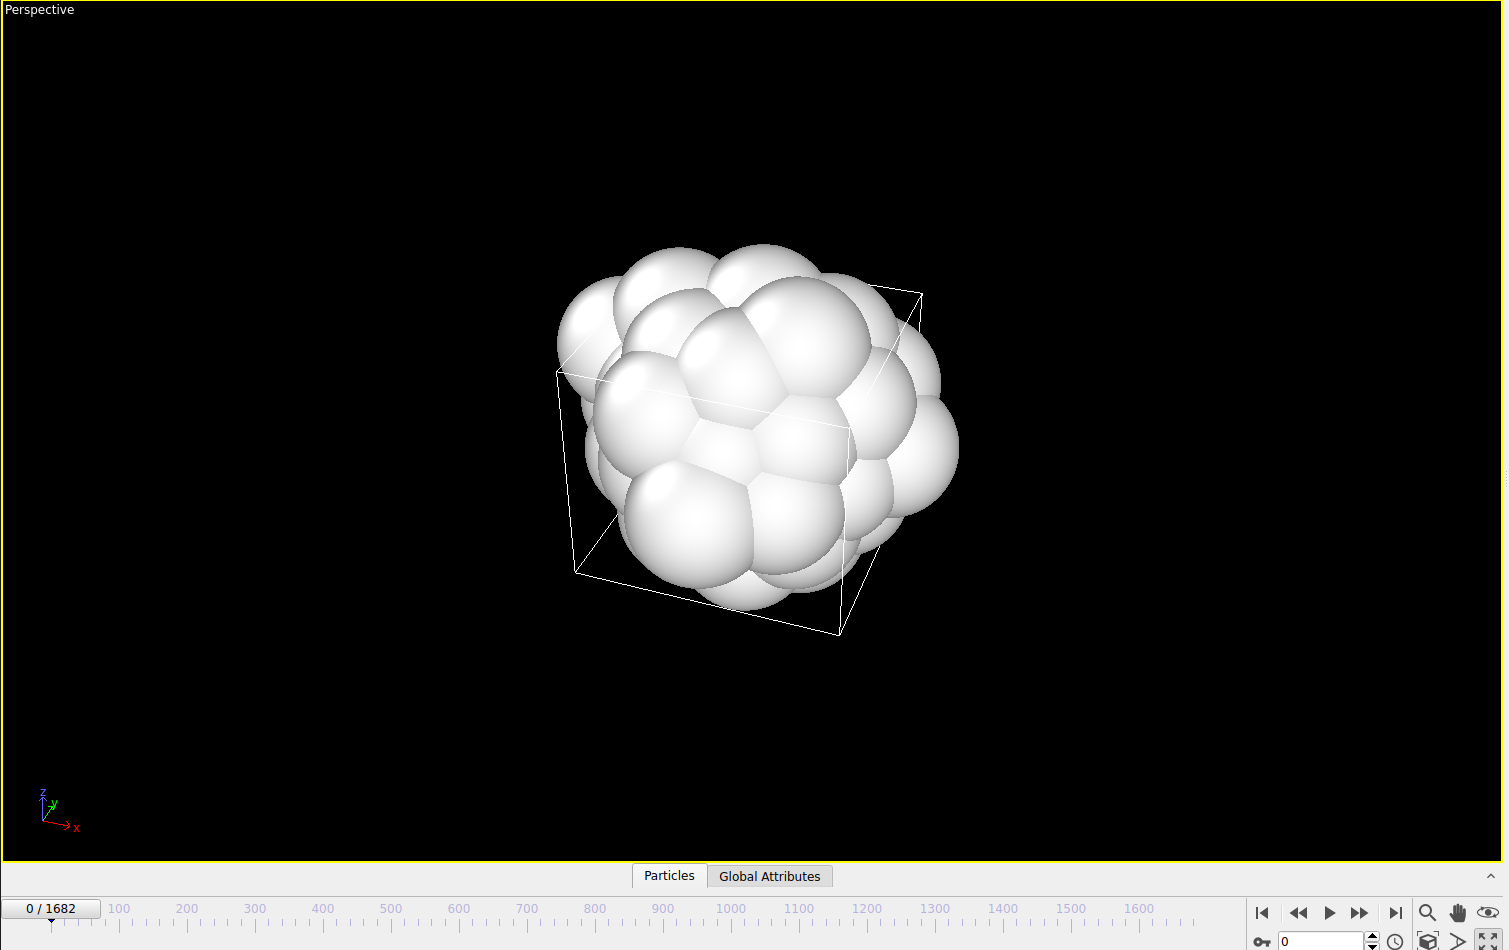
\includegraphics[scale=0.25]{ML1.png}
        \caption{LJ simulation snapshot1}
    \label{fig:step1}
    \end{figure}
    \begin{figure}[!htb]
    \centering
        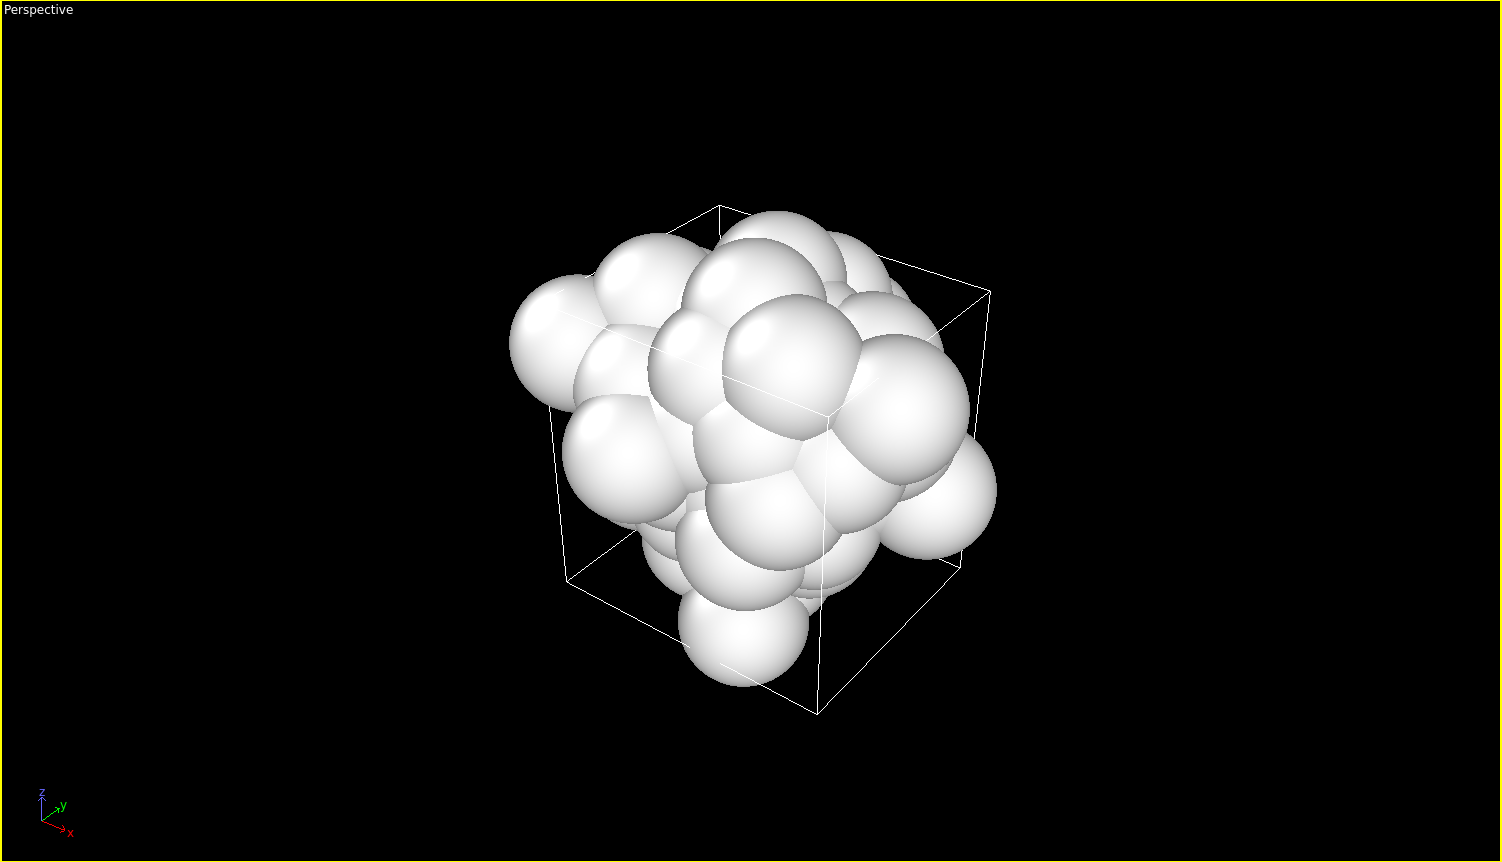
\includegraphics[scale=0.25]{ML2.png}
        \caption{LJ simulation snapshot2}
    \label{fig:step2}
    \end{figure}
    \begin{figure}[!htb]
    \centering
        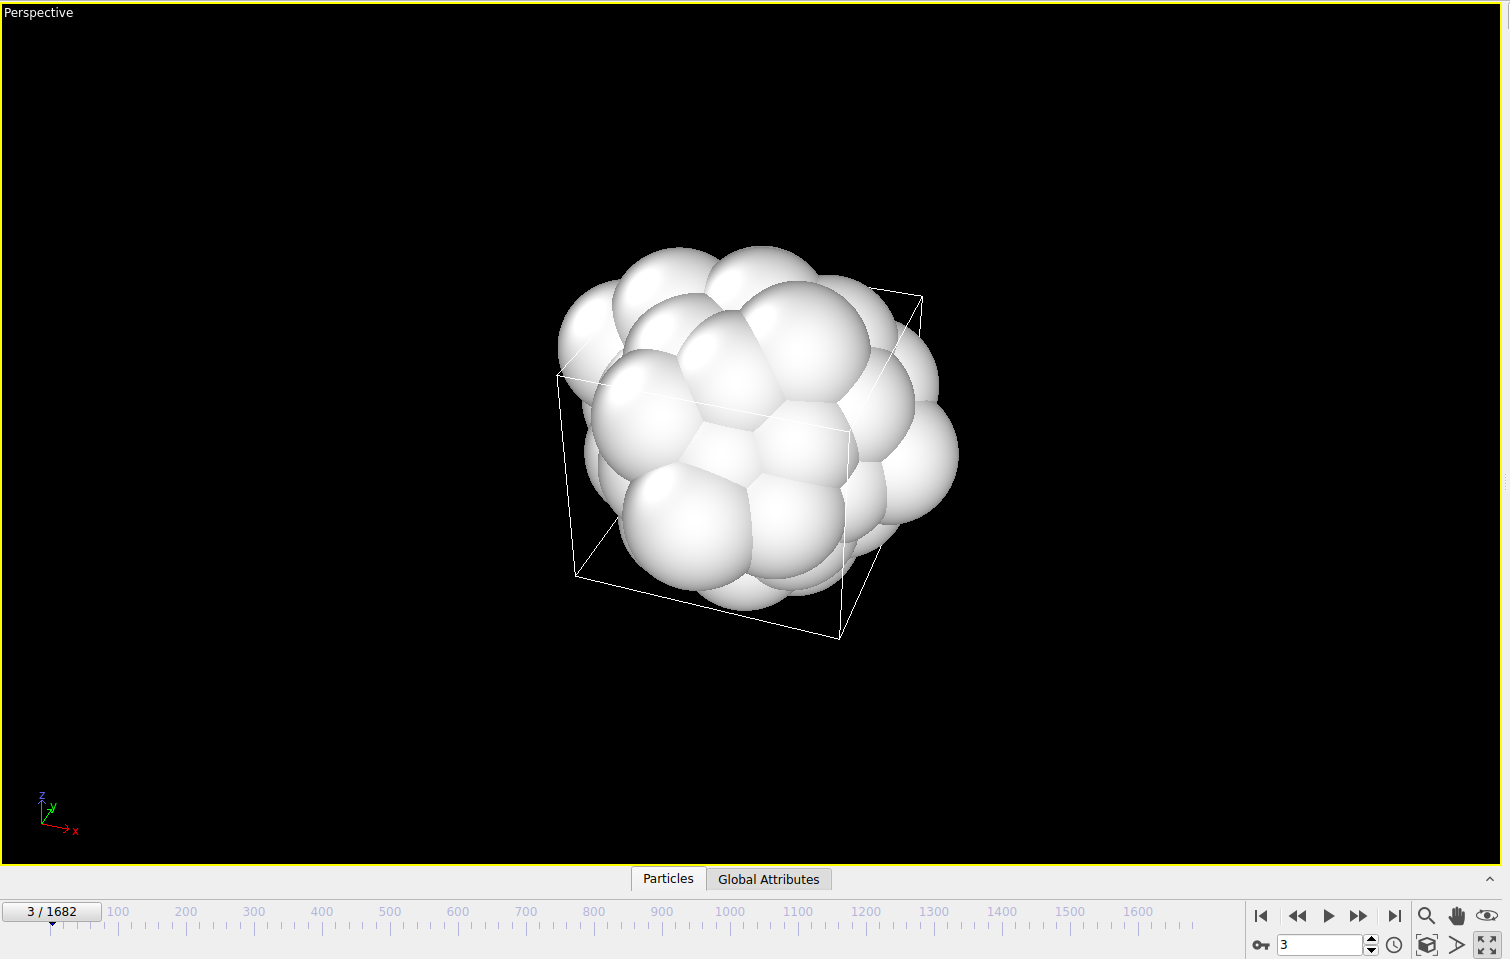
\includegraphics[scale=0.25]{ML3.png}
        \caption{LJ simulation snapshot3}
    \label{fig:step3}
    \end{figure}
    \begin{figure}[!htb]
    \centering
        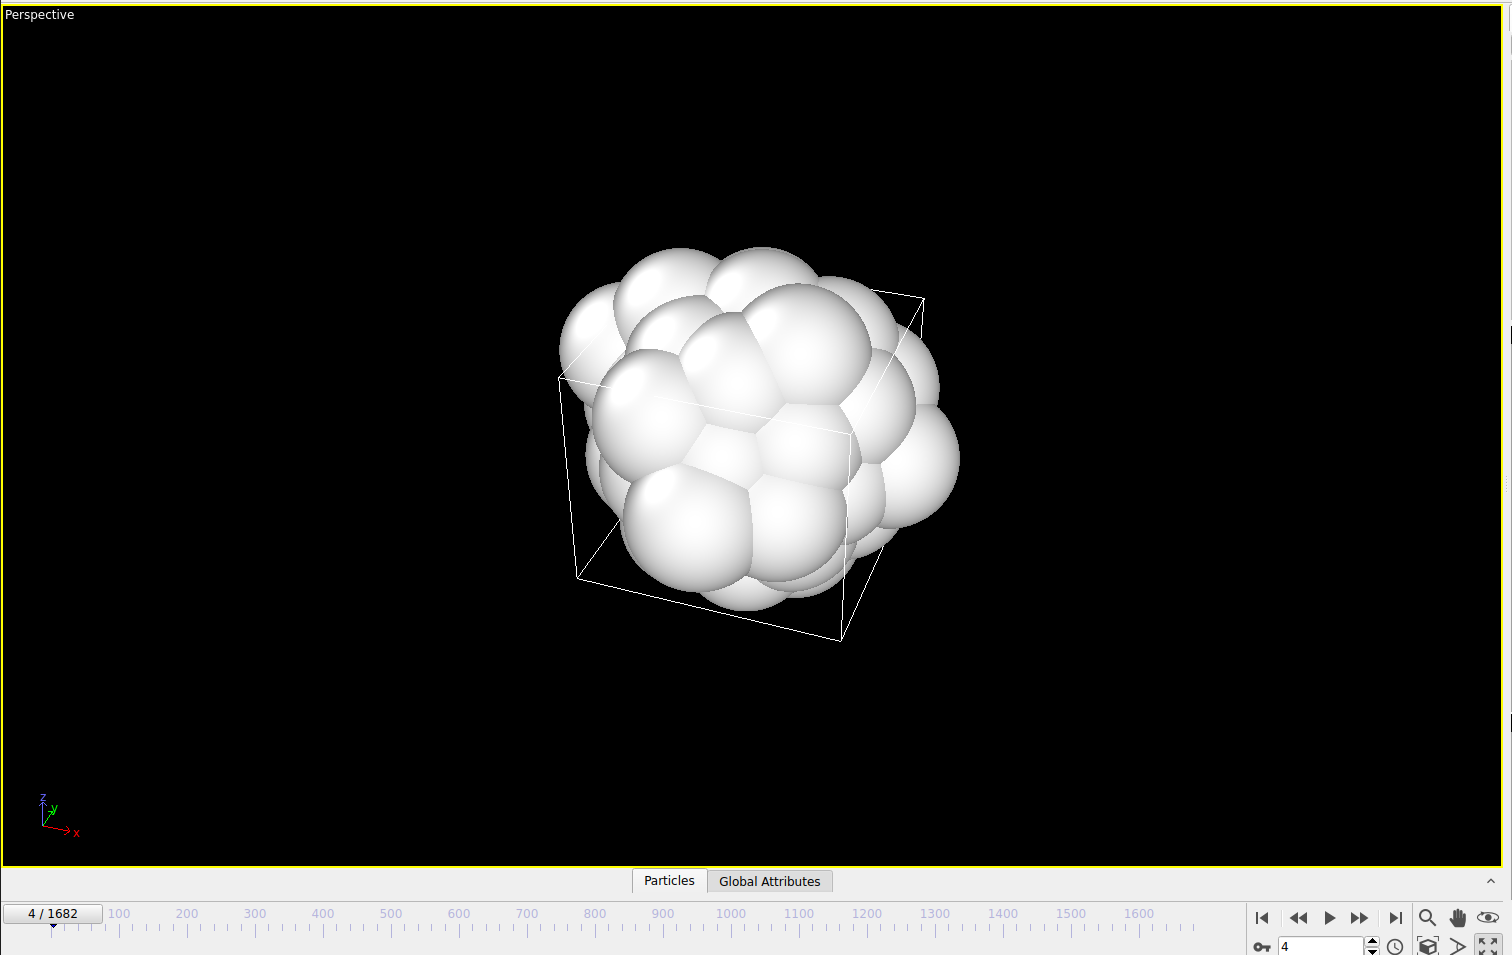
\includegraphics[scale=0.25]{ML4.png}
        \caption{LJ simulation snapshot4}
    \label{fig:step4}
    \end{figure}
    \begin{figure}[!htb]
    \centering
        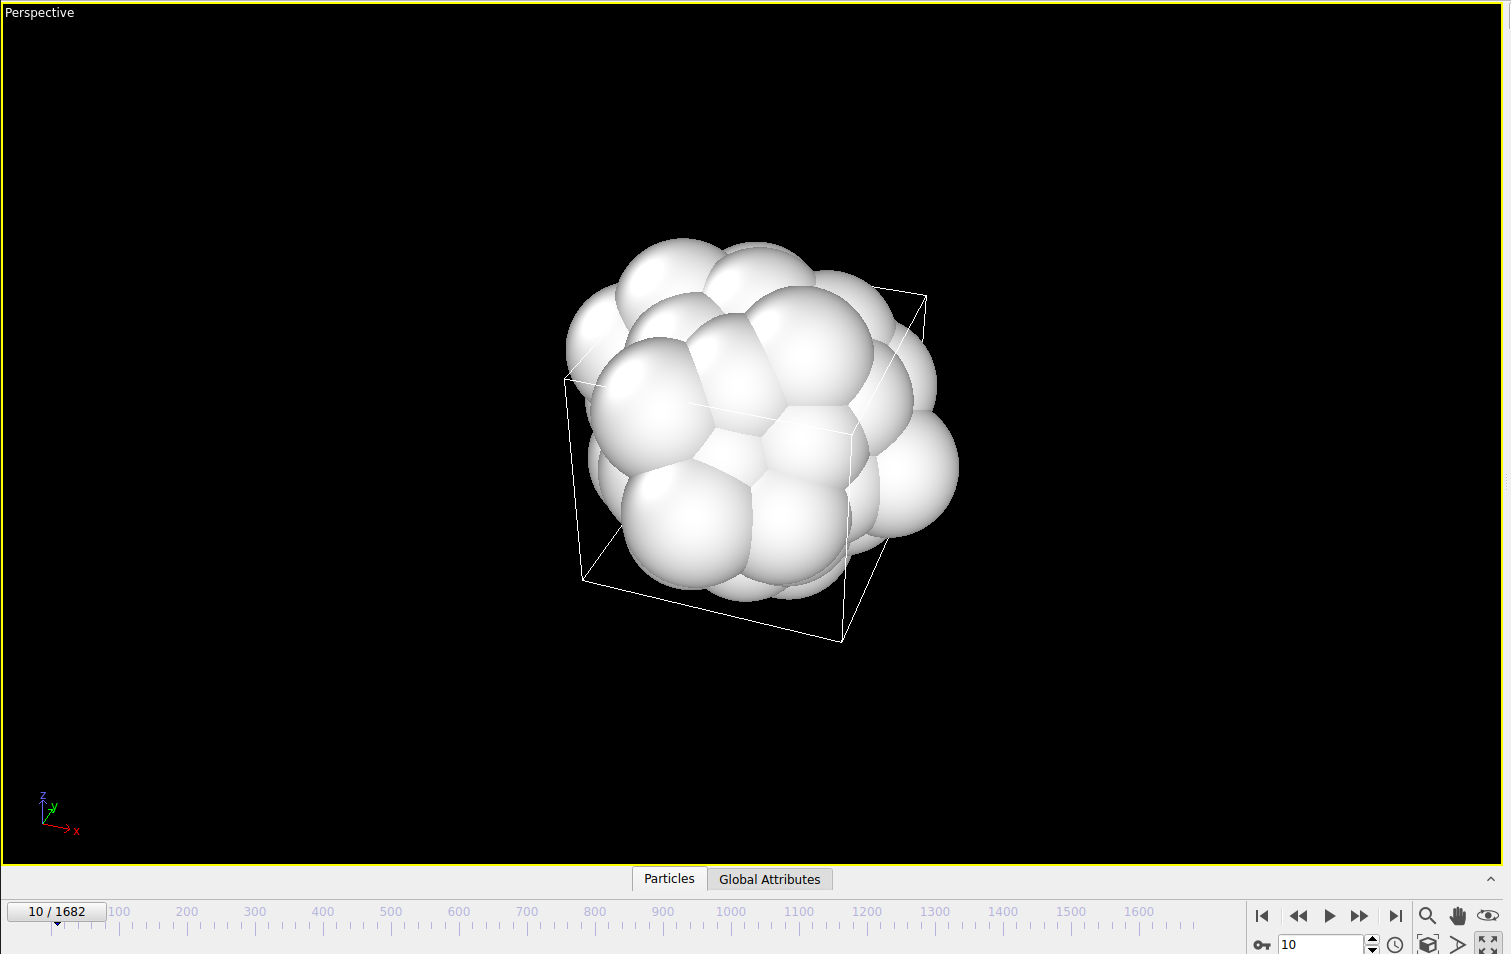
\includegraphics[scale=0.25]{ML5.png}
        \caption{LJ simulation snapshot5}
    \label{fig:step5}
    \end{figure}



\section{simulation time as a function of the size (number of atoms) without neighbor list}
\section{simulation time as a function of the size (number of atoms) with neighbor list}

\section{total energy vs temperature}
\section{melting point versus cluster size}
\section{heat capacity versus cluster size}
\section{latent heat versus cluster size}
\section{Energy conservation with MPI parallelization}
% \section{Nanowire σ/ɛ}
\section{Nanowire defects}